\documentclass[en,16:9,navbarinline,bigfoot]{sdqbeamer} 
\usepackage[spanish]{babel}
\usepackage{booktabs}
\usepackage{rotating}
 
\titleimage{duv_stepper_working}

\groupname{Maestría en Ciencias de la Ingeniería Eléctrica}
\groupnamewidth{75mm}

\title[LGAC en Mecatrónica]{Optimización de Trayectorias de Orden Superior Informadas por el Rendimiento de la Oblea para Sistemas \textit{Step-and-Scan}}
\subtitle{Seminario I}
\author[R. Treviño]{Roberto Treviño Cervantes}
\newcommand{\shorttoday}{\ifnum\day<10 0\fi\number\day/\ifnum\month<10 0\fi\number\month/\number\year}
\date[\shorttoday]{\today}

\usepackage[citestyle=authoryear,bibstyle=numeric,hyperref,backend=biber,maxnames=1]{biblatex}
\addbibresource{presentation.bib}
\bibhang1em

\usepackage{tikz}
\usetikzlibrary{decorations.pathmorphing,decorations.pathreplacing,patterns,arrows.meta,calc,positioning,3d,fit,shapes.geometric}
\usepackage{import}
\subimport{../PlotNeuralNet/layers/}{init}

\def\ConvColor{rgb:yellow,5;red,2.5;white,5}
\def\ConvReluColor{rgb:yellow,5;red,5;white,5}
\def\PoolColor{rgb:red,1;black,0.3}
\def\UnpoolColor{rgb:blue,2;green,1;black,0.3}
\def\FcColor{rgb:blue,5;red,2.5;white,5}
\def\FcReluColor{rgb:blue,5;red,5;white,4}
\def\SoftmaxColor{rgb:magenta,5;black,7}

%%%%%%% ---- COLOR PALETTE --------
\definecolor{mnnwInk}     {HTML}{0A0A0A}
\definecolor{mnnwSignal}  {HTML}{0A84FF}
\definecolor{mnnwHair}    {HTML}{C9C9C9}
\definecolor{mnnwMute}    {HTML}{6F6F6F}
\definecolor{reticleFill} {HTML}{DCE6F7}  
\definecolor{reticleEdge} {HTML}{4F6F9F}
\definecolor{reticleFlex} {HTML}{EEF3FB}  
\definecolor{waferFill}   {HTML}{F5DCDC}  
\definecolor{waferEdge}   {HTML}{9F4F4F}
\definecolor{waferFlex}   {HTML}{FBEEEE}
\definecolor{opticsFill}  {HTML}{E7DCF5}  
\definecolor{opticsEdge}  {HTML}{6F4F9F}
\definecolor{opticsFlex}  {HTML}{F3EEFB}
\definecolor{frameFill}   {HTML}{D9E8D2}  
\definecolor{frameEdge}   {HTML}{4F7F3F}
\definecolor{lensFill}    {HTML}{EEEEEE}

\tikzset{
  hdamper/.pic={
    \draw[line width=0.5pt, mnnwInk] (-0.45,0)            -- (-0.18,0);
    \draw[line width=0.5pt, mnnwInk] (-0.18,-0.11) rectangle (0.18,0.11);
    \draw[line width=0.5pt, mnnwInk] (0,-0.11)            -- (0,0.11);
    \draw[line width=0.5pt, mnnwInk] (0.18,0)             -- (0.45,0);
  },
  vdamper/.pic={
    \draw[line width=0.5pt, mnnwInk] (0,-0.45)            -- (0,-0.18);
    \draw[line width=0.5pt, mnnwInk] (-0.11,-0.18) rectangle (0.11,0.18);
    \draw[line width=0.5pt, mnnwInk] (-0.11,0)            -- (0.11,0);
    \draw[line width=0.5pt, mnnwInk] (0,0.18)             -- (0,0.45);
  },
}
\newcommand{\hdamperLong}[3]{%
  \pgfmathsetmacro{\xa}{#1}\pgfmathsetmacro{\xb}{#2}\pgfmathsetmacro{\yy}{#3}
  \pgfmathsetmacro{\Lcyl}{(\xb-\xa)*0.55}
  \pgfmathsetmacro{\xcylR}{\xa+\Lcyl}
  \pgfmathsetmacro{\xpisR}{\xb}
  \draw[line width=0.5pt, mnnwInk] (\xa,\yy-0.13) -- (\xa,\yy+0.13);
  \draw[line width=0.5pt, mnnwInk] (\xa,\yy+0.13) -- (\xcylR,\yy+0.13);
  \draw[line width=0.5pt, mnnwInk] (\xa,\yy-0.13) -- (\xcylR,\yy-0.13);
  \pgfmathsetmacro{\xpiston}{\xa+\Lcyl*0.70}
  \draw[line width=0.5pt, mnnwInk] (\xpiston,\yy-0.11) -- (\xpiston,\yy+0.11);
  \draw[line width=0.5pt, mnnwInk] (\xpiston,\yy) -- (\xpisR,\yy);
}
\newcommand{\vdamperLong}[3]{%
  \pgfmathsetmacro{\xx}{#1}\pgfmathsetmacro{\ya}{#2}\pgfmathsetmacro{\yb}{#3}
  \pgfmathsetmacro{\Lcyl}{(\yb-\ya)*0.55}
  \pgfmathsetmacro{\ycylT}{\ya+\Lcyl}
  \draw[line width=0.5pt, mnnwInk] (\xx-0.13,\ya) -- (\xx+0.13,\ya);
  \draw[line width=0.5pt, mnnwInk] (\xx-0.13,\ya) -- (\xx-0.13,\ycylT);
  \draw[line width=0.5pt, mnnwInk] (\xx+0.13,\ya) -- (\xx+0.13,\ycylT);
  \pgfmathsetmacro{\ypiston}{\ya+\Lcyl*0.70}
  \draw[line width=0.5pt, mnnwInk] (\xx-0.11,\ypiston) -- (\xx+0.11,\ypiston);
  \draw[line width=0.5pt, mnnwInk] (\xx,\ypiston) -- (\xx,\yb);
}

\def\getfirstchar#1#2\relax{#1}
\newcommand{\chainrow}[8]{%
  \edef\styleName{#2}%
  \def\currColor{mnnwMute}%
  \edef\firstChar{\expandafter\getfirstchar\styleName\relax}%
  \if\firstChar w\def\currColor{waferEdge}\fi
  \if\firstChar o\def\currColor{opticsEdge}\fi
  \if\firstChar r\def\currColor{reticleEdge}\fi
  \pgfmathparse{abs(#3 - \lastX) < 0.001 ? 1 : 0}
  \ifnum\pgfmathresult=1
    \pgfmathparse{abs(#3) < 0.001 ? 1 : 0}
    \ifnum\pgfmathresult=1 \def\lineColor{frameEdge} \else \def\lineColor{\currColor} \fi
    \draw[line width=0.35pt, \lineColor] (#3, \lastSpringY) -- (#3, #1-0.62);
  \fi
  \node[#2, inner xsep=6pt] (blk) at (#4,#1) {#5};
  \node[ghost, inner xsep=6pt] at (#3,#1) {\phantom{#5}};
  \draw[hsp] (#3, #1+0.62) -- (#4, #1+0.62);
  \draw[line width=0.35pt, mnnwInk] (#3, #1+0.275) -- (#3, #1+0.62);
  \draw[line width=0.35pt, mnnwInk] (#4, #1+0.275) -- (#4, #1+0.62);
  \draw[line width=0.35pt, mnnwInk] (#3, #1-0.275) -- (#3, #1-0.62);
  \draw[line width=0.35pt, mnnwInk] (#4, #1-0.275) -- (#4, #1-0.62);
  \hdamperLong{#3}{#4}{#1-0.62}
  \pgfmathsetmacro{\lblSide}{#4 > #3 ? #3 : #3}
  \pgfmathsetmacro{\lblAnch}{#4 > #3 ? "east" : "west"}
  \node[lbl, anchor=\lblAnch] at (\lblSide, #1+0.62) {#6}; 
  \node[lbl, anchor=\lblAnch] at (\lblSide, #1-0.62) {#7}; 
  \pgfmathsetmacro{\fSide}{#4 > #3 ? #4 : #4}
  \pgfmathsetmacro{\fAnch}{#4 > #3 ? "west" : "east"}
  \node[ftn, anchor=\fAnch] at (\fSide, #1-0.525) {#8};
  \draw[darr] (#3, #1-0.275) -- (#4, #1-0.275);
  \pgfmathsetmacro{\newSpringY}{#1+0.62}
  \xdef\lastSpringY{\newSpringY}
  \pgfmathsetmacro{\newX}{#4}
  \xdef\lastX{\newX}
}

%% Logo and Layout Settings
\kitlogo{uanl}
\grouplogo{fime}
\kitslogan{}

% Custom Title Frame Command to replace \KITtitleframe
\newcommand{\UANLtitleframe}{%
  \begin{frame}[plain]
    % Larger logos for the title page only
    \begin{textblock*}{18mm}(7.3mm,6.7mm)
      
\includegraphics[width=18mm]{logos/uanl.eps}%
    \end{textblock*}%
    \begin{textblock*}{22mm}(\dimexpr\paperwidth-22.3mm\relax,6.7mm)
      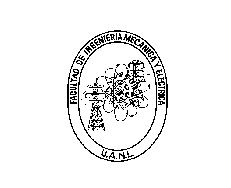
\includegraphics[width=22mm,height=22mm,keepaspectratio]{logos/fime.eps}%
    \end{textblock*}%
    \begin{textblock*}{\dimexpr\paperwidth-2\kitinnermargin\relax}[0,.5](7.3mm,35mm)
      {\usebeamerfont{title}\inserttitle}%
    \end{textblock*}%
    \begin{textblock*}{\dimexpr\paperwidth-2\kitinnermargin\relax}[0,.5](7.3mm,45mm)
      {\usebeamerfont{subtitle}\insertsubtitle}%
    \end{textblock*}%
    \begin{textblock*}{\dimexpr\paperwidth-2\kitinnermargin\relax}[0,.5](7.3mm,52mm)
      {\usebeamerfont{author}\insertauthor\ \textbar\ \insertdate}%
    \end{textblock*}%
    \begin{textblock*}{\paperwidth}(2mm,60mm)
      \centering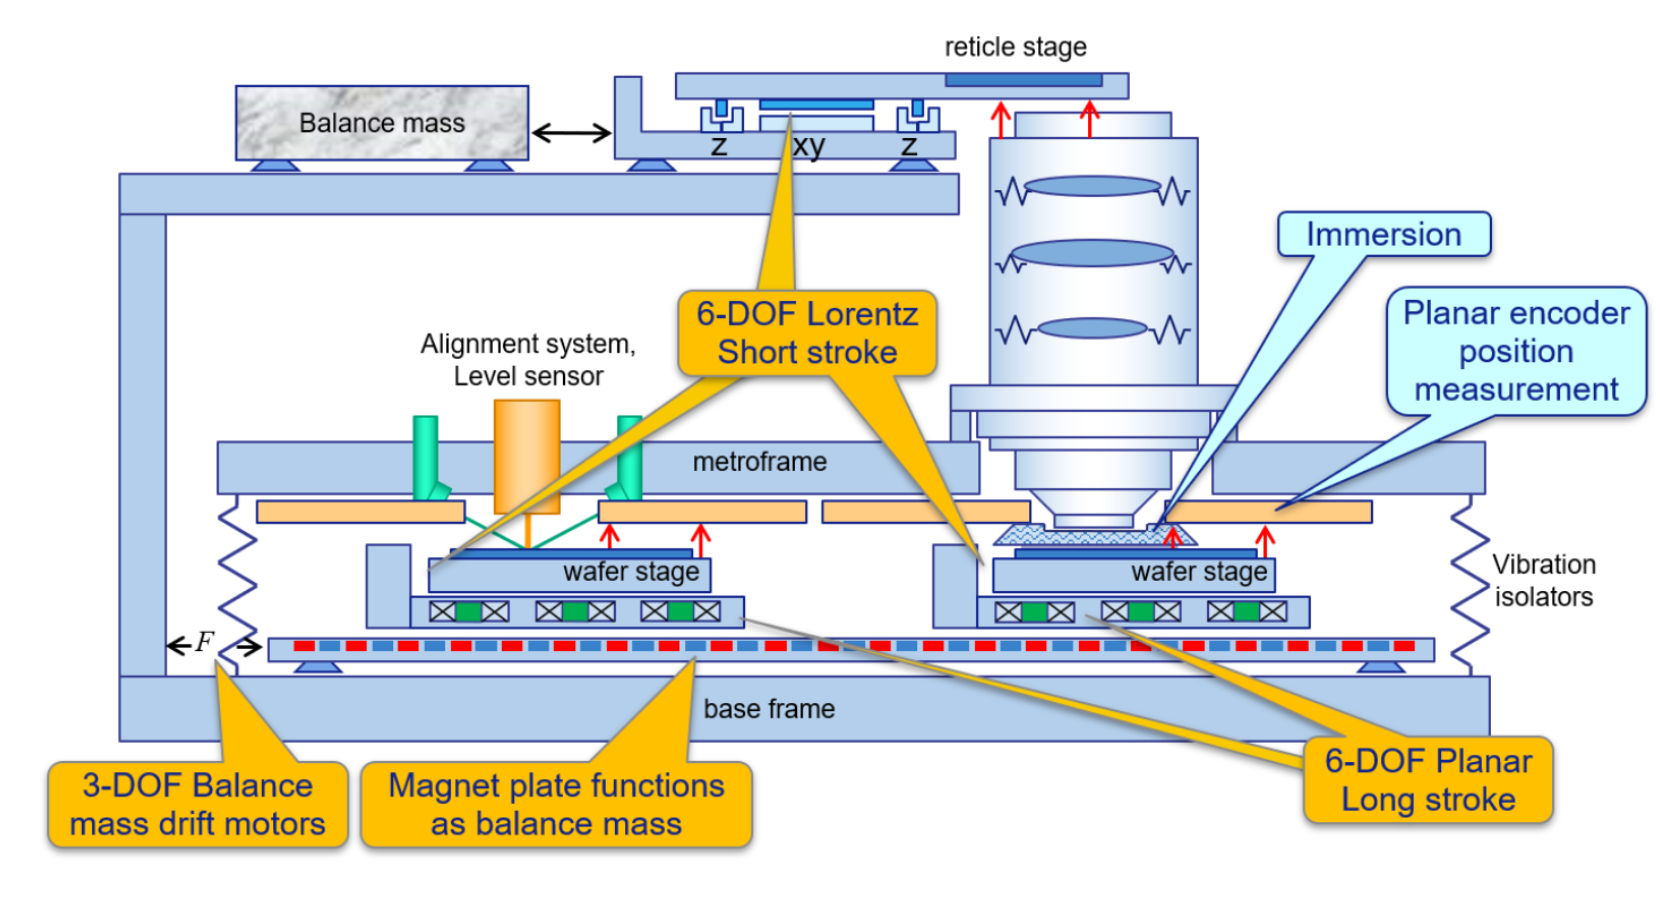
\includegraphics[height=30mm]{logos/metroframe-etc.png}%
    \end{textblock*}%
  \end{frame}
}

% Simplified tiny side-by-side logos for frametitle
\setbeamertemplate{frametitle}{%
  \begin{textblock*}{120mm}[0,1](7.3mm,15mm)
    {\usebeamerfont{frametitle}\insertframetitle}%
  \end{textblock*}%
  \begin{textblock*}{12mm}[1,1](\dimexpr\paperwidth-12.3mm\relax,15mm)
    
\includegraphics[width=8mm]{logos/uanl.eps}%
  \end{textblock*}%
  \begin{textblock*}{8mm}[1,1](\dimexpr\paperwidth-7.3mm\relax,15mm)
    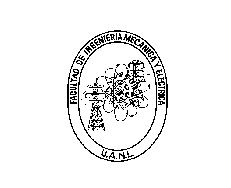
\includegraphics[width=10mm]{logos/fime.eps}%
  \end{textblock*}%
  \vspace{18mm}
}

\begin{document}

\UANLtitleframe

\begin{frame}{Índice}
\tableofcontents
\end{frame}

\section{Introducción a la Fabricación de Circuitos Integrados}

\begin{frame}{Fabricación de Circuitos Integrados}
    \begin{center}
        \begin{tikzpicture}[scale=0.92, transform shape, every node/.style={font=\footnotesize}]
            % Photolithography Process Diagram
            \draw[fill=kit-yellow50, draw=mnnwInk] (-0.5, 5.0) rectangle (0.5, 4.6);
            \node[anchor=west] at (0.6, 4.8) {Fuente de luz};

            % Reticle
            \draw[fill=reticleFill, draw=reticleEdge] (-1.8, 3.4) rectangle (1.8, 3.1);
            \draw[draw=kit-red100, -{Stealth[scale=1.2]}, line width=1.5pt] (1.2, 3.7) -- (-1.2, 3.7) node[left, font=\footnotesize\bfseries] {$\mathbf{v}_r$};
            \node[anchor=west] at (1.9, 3.25) {Fotomáscara};

            % Lens
            \draw[fill=lensFill, draw=mnnwInk] (0, 1.8) ellipse (1.2cm and 0.25cm);
            \node[anchor=west] at (1.3, 1.8) {Lente};

            % Wafer with detailed dies
            \begin{scope}
                \clip (0, 0) ellipse (2.2cm and 0.45cm);
                \fill[waferFill] (-2.2, -0.45) rectangle (2.2, 0.45);
                \foreach \x in {-2.0,-1.75,...,2.0} {
                    \foreach \y in {-0.3, -0.15, 0, 0.15, 0.3} {
                        \draw[draw=waferEdge!40, line width=0.05pt] (\x-0.08, \y-0.06) rectangle (\x+0.08, \y+0.06);
                    }
                }
            \end{scope}
            \draw[fill=none, draw=waferEdge] (0, 0) ellipse (2.2cm and 0.45cm);
            \draw[draw=kit-blue100, -{Stealth[scale=1.2]}, line width=1.5pt] (-1.2, -0.75) -- (1.2, -0.75) node[right, font=\footnotesize\bfseries] {$\mathbf{v}_w$};
            \node[anchor=west] at (2.3, 0) {Oblea};

            % Light Beams
            \draw[draw=mnnwSignal, line width=0.8pt, opacity=0.3] (0, 4.6) -- (0, 3.4);
            \draw[draw=mnnwSignal, line width=0.8pt, opacity=0.3] (0, 3.1) -- (0, 2.05);
            \draw[draw=mnnwSignal!80!black, line width=1.2pt, opacity=0.7] (0, 1.55) -- (0, 0.1);

            % Callouts: CD and Moore
            \node[anchor=west, font=\small\bfseries, text=kit-red100] at (-5.6, 4.8) {Ley de Moore};
            \node[anchor=west, font=\footnotesize, text=mnnwInk] at (-5.6, 4.35) {$\downarrow$ tamaño exponencial};
            \node[anchor=west, font=\small\bfseries, text=kit-blue100] at (-5.6, 0.4) {CD};
            \node[anchor=west, font=\footnotesize] at (-5.6, -0.05) {18\,nm EUV};
            \node[anchor=west, font=\footnotesize] at (-5.6, -0.45) {38\,nm DUV};
        \end{tikzpicture}
    \end{center}
\end{frame}

\begin{frame}[fragile]{El Proceso \textit{Step-and-Scan}}
    \begin{center}
          \begin{tikzpicture}[scale=1.3,
            every node/.style={font=\footnotesize},
            wafer/.style={draw=kit-blue100, line width=0.6pt, fill=kit-blue!5},
            die/.style={draw=mnnwInk, line width=0.3pt, fill=white, postaction={pattern=north east lines, pattern color=mnnwMute!40}},
            scan/.style={draw=kit-red100, line width=0.8pt, dashed, -{Stealth[scale=0.5]}},
            stepArrow/.style={draw=kit-lightgreen100, line width=0.8pt, -{Stealth[scale=0.5]}},
            traverse/.style={draw=mnnwInk, line width=0.5pt, dotted, -{Stealth[scale=0.5]}},
            point/.style={circle, fill=kit-blue100, inner sep=1pt}
          ]
            
            % Wafer boundary
            \draw[wafer] (0,0) circle (2.2cm);
            
            % Grid of dies clipped to wafer
            \begin{scope}
              \clip (0,0) circle (2.2cm);
              \foreach \x in {-1.75,-1.25,...,1.75} {
                \foreach \y in {-1.75,-1.25,...,1.75} {
                  \draw[die] (\x-0.2,\y-0.2) rectangle (\x+0.2,\y+0.2);
                }
              }
            \end{scope}

            % 2: Scan Up
            \draw[scan] (-1.25, -1.75) -- (-1.25, -1.25) node[midway, left, text=kit-red100] {};
            
            % 3: Step Right (to Column 2)
            \draw[stepArrow] (-1.25, -1.25) -- (-0.75, -1.25) node[midway, above, text=kit-lightgreen100] {};
            
            % 4: Scan Down (Column 2)
            \draw[scan] (-0.75, -1.25) -- (-0.75, -1.75) node[midway, right, text=kit-red100] {};
            
            % 5: Step Right (to Column 3)
            \draw[stepArrow] (-0.75, -1.75) -- (-0.25, -1.75) node[midway, below, text=kit-lightgreen100] {};
            
            % 6: Scan Up (Column 3)
            \draw[scan] (-0.25, -1.75) -- (-0.25, -1.25) node[midway, left, text=kit-red100] {};
            
            % 7: Step Right (to Column 4)
            \draw[stepArrow] (-0.25, -1.25) -- (0.25, -1.25) node[midway, above, text=kit-lightgreen100] {};
            
            % 8: Scan Down (Column 4)
            \draw[scan] (0.25, -1.25) -- (0.25, -1.75) node[midway, right, text=kit-red100] {};
            
            % Axes
            \draw[draw=mnnwInk, -Stealth] (0,0) -- (0.4,0) node[right] {$x$};
            \draw[draw=mnnwInk, -Stealth] (0,0) -- (0,0.4) node[above] {$y$};

            % Legend: scan / step / velocity ratio
            \node[anchor=west, font=\footnotesize, text=kit-red100] at (2.6, 1.8) {-- -- \textbf{scan}};
            \node[anchor=west, font=\footnotesize, text=kit-lightgreen100] at (2.6, 1.3) {$\to$ \textbf{step}};
            \node[anchor=west, font=\footnotesize] at (2.6, 0.6) {$v_r = 4\,v_w$};
            \node[anchor=west, font=\footnotesize] at (2.6, 0.1) {sentidos opuestos};

          \end{tikzpicture}
        \end{center}
\end{frame}

\begin{frame}{\textit{Overlay} y productividad}
    \begin{columns}[T]
        \column{.5\textwidth}
        \begin{blueblock}{\textit{Overlay} (nm)}
            Desviación entre las múltiples capas de un IC; debe minimizarse para asegurar la interconexión (\cite{Schmidt2012_UltraPrecision}).
        \end{blueblock}

        \column{.5\textwidth}
        \begin{greenblock}{Productividad (obleas por hora)}
            Producción continua de alto volumen (\cite{Butler2011_PositionControl}).
        \end{greenblock}
    \end{columns}

    \vspace{0.05cm}
    \begin{center}
    \begin{tikzpicture}[scale=0.72, transform shape, every node/.style={font=\footnotesize}]

        % =========================================================
        % PANEL A — Overlay correcto
        % =========================================================
        \node[font=\small\bfseries, anchor=south] at (3.0, 4.20) {Overlay correcto};

        % Top view: 2x2 grid, match — 4 red horizontals + 4 blue verticals, same positions
        \begin{scope}[shift={(2.08, 2.25)}]
            \foreach \i in {0,1} {
                \foreach \j in {0,1} {
                    \begin{scope}[shift={(\i*0.95, \j*0.95)}]
                        \fill[white] (0,0) rectangle (0.90, 0.90);
                        \foreach \y in {0.076, 0.282, 0.488, 0.694} {
                            \fill[kit-red100, fill opacity=0.85] (0.04, \y) rectangle (0.86, \y+0.13);
                        }
                        \foreach \x in {0.076, 0.282, 0.488, 0.694} {
                            \fill[kit-blue100, fill opacity=0.60] (\x, 0.04) rectangle (\x+0.13, 0.86);
                        }
                        \draw[draw=mnnwHair, line width=0.3pt] (0,0) rectangle (0.90, 0.90);
                    \end{scope}
                }
            }
        \end{scope}

        \draw[draw=mnnwMute, line width=1.1pt, -Stealth] (3.0, 2.20) -- (3.0, 1.70);

        % Cross-section: P bars aligned with Q (match)
        \begin{scope}[shift={(1.3, 0.50)}]
            \fill[kit-green100!85]      (0, 0)    rectangle (3.4, 0.16);
            \fill[kit-lightgreen100!35] (0, 0.16) rectangle (3.4, 0.58);
            \foreach \x in {0.40, 0.92, 1.44, 1.96, 2.48, 3.00} {
                \fill[kit-red100] (\x-0.12, 0.19) rectangle (\x+0.12, 0.38);
            }
            \foreach \x in {0.40, 0.92, 1.44, 1.96, 2.48, 3.00} {
                \fill[kit-blue100] (\x-0.12, 0.62) rectangle (\x+0.12, 0.81);
            }
            \node[anchor=west, font=\footnotesize, text=kit-blue100] at (3.50, 0.71) {Capa actual, P};
            \node[anchor=west, font=\footnotesize, text=kit-red100]  at (3.50, 0.28) {Capa previa, Q};
        \end{scope}

        % =========================================================
        % PANEL B — Error de overlay
        % =========================================================
        \begin{scope}[shift={(6.5, 0)}]
            \node[font=\small\bfseries, anchor=south] at (3.0, 4.20) {Error de \textit{overlay}};

            % Top view: same 4 red horizontals; blue verticals shifted by half-period
            \begin{scope}[shift={(2.08, 2.25)}]
                \foreach \i in {0,1} {
                    \foreach \j in {0,1} {
                        \begin{scope}[shift={(\i*0.95, \j*0.95)}]
                            \fill[white] (0,0) rectangle (0.90, 0.90);
                            \foreach \y in {0.076, 0.282, 0.488, 0.694} {
                                \fill[kit-red100, fill opacity=0.85] (0.04, \y) rectangle (0.86, \y+0.13);
                            }
                            \begin{scope}
                                \clip (0,0) rectangle (0.90, 0.90);
                                \foreach \x in {0.178, 0.384, 0.590, 0.796} {
                                    \fill[kit-blue100, fill opacity=0.60] (\x, 0.04) rectangle (\x+0.13, 0.86);
                                }
                            \end{scope}
                            \draw[draw=mnnwHair, line width=0.3pt] (0,0) rectangle (0.90, 0.90);
                        \end{scope}
                    }
                }
            \end{scope}

            \draw[draw=mnnwMute, line width=1.1pt, -Stealth] (3.0, 2.20) -- (3.0, 1.70);

            % Cross-section: P bars shifted by half-period from Q (mismatch)
            \begin{scope}[shift={(1.3, 0.50)}]
                \fill[kit-green100!85]      (0, 0)    rectangle (3.4, 0.16);
                \fill[kit-lightgreen100!35] (0, 0.16) rectangle (3.4, 0.58);
                \foreach \x in {0.40, 0.92, 1.44, 1.96, 2.48, 3.00} {
                    \fill[kit-red100] (\x-0.12, 0.19) rectangle (\x+0.12, 0.38);
                }
                \foreach \x in {0.66, 1.18, 1.70, 2.22, 2.74, 3.26} {
                    \fill[kit-blue100] (\x-0.12, 0.62) rectangle (\x+0.12, 0.81);
                }
                \node[anchor=west, font=\footnotesize, text=kit-blue100] at (3.50, 0.71) {Capa actual, P};
                \node[anchor=west, font=\footnotesize, text=kit-red100]  at (3.50, 0.28) {Capa previa, Q};
            \end{scope}
        \end{scope}

    \end{tikzpicture}
    \end{center}
\end{frame}

\begin{frame}[t,fragile]{Antecedentes --- análisis de literatura}
    \footnotesize PRISMA 2020--2025 $\cdot$ 1\,180 cribados $\to$ 12 incluidos $\cdot$ póster IEEE LARS/LARC 2025 (\cite{Trevino2025_LARSPoster}).

    \vspace{0.1cm}
    \begin{center}
    \begin{tikzpicture}[every node/.style={font=\footnotesize}]
        \def\barH{0.26}
        \def\unit{0.68}
        \foreach \name/\cnt/\col [count=\i] in {%
            {\textit{Input shaping}}/3/kit-red100,
            {Control basado en datos}/3/opticsEdge,
            {Sincronización de cadenas}/2/kit-blue100,
            {Modelado predictivo}/2/kit-lightgreen100,
            {Control adaptativo}/1/waferEdge,
            {Redes neuronales}/1/kit-yellow!75!black%
        }{
            \pgfmathsetmacro{\y}{-\i*0.48}
            \node[anchor=east, font=\footnotesize] at (0,\y) {\name};
            \fill[\col] (0.15,\y-\barH/2) rectangle ({0.15+\cnt*\unit},\y+\barH/2);
            \node[anchor=west, font=\footnotesize, text=mnnwInk] at ({0.22+\cnt*\unit},\y) {\cnt};
        }
        \node[anchor=west, font=\scriptsize, text=mnnwMute] at (0.15,-3.30) {reportes incluidos (n{=}12)};
    \end{tikzpicture}
    \end{center}
    \vspace{0.05cm}
    \begin{purpleblock}{Brecha}
        \footnotesize Métricas \textbf{servo-mecánicas} (MSE) sin considerar el impacto \textbf{morfológico} en el \textit{yield}; análisis inverso de \textit{fingerprints} (\cite{Lam2015_Fingerprint}) no cubre la dirección directa.
    \end{purpleblock}
\end{frame}

\begin{frame}[fragile]{Hipótesis y objetivos}
    \begin{purpleblock}{Hipótesis}
        Una CNN entrenada sobre WM-811K, usada como función de costo, permite seleccionar parámetros cinemáticos de trayectorias de cuarto orden que \textbf{minimicen la probabilidad de defecto} sujeto a una \textbf{restricción de productividad}.
    \end{purpleblock}

    \vspace{0.3cm}
    \begin{center}
    \begin{tikzpicture}[
        every node/.style={font=\footnotesize},
        obj/.style={draw=opticsEdge, line width=0.7pt, rounded corners=2pt, fill=opticsFlex, minimum width=2.9cm, minimum height=1.5cm, align=center},
        ar/.style={-Stealth, line width=0.9pt, opticsEdge}
    ]
        \node[obj] (a) {\textbf{1.}\\Generar trayectorias\\acotadas en \textit{snap}};
        \node[obj, right=0.6cm of a] (b) {\textbf{2.}\\Entrenar CNN\\sobre WM-811K};
        \node[obj, right=0.6cm of b] (c) {\textbf{3.}\\Usar CNN como\\función de costo};
        \draw[ar] (a) -- (b);
        \draw[ar] (b) -- (c);
    \end{tikzpicture}
    \end{center}
\end{frame}

\section{Modelo}

\begin{frame}[fragile]{Sistema multicuerpo}
    \begin{center}
        \begin{tikzpicture}[scale=0.55, every node/.style={font=\footnotesize}]
            % Canvas: 14 wide x 8.6 tall (tightened)
            \draw[draw=frameEdge!70, line width=0.8pt, rounded corners=4pt]
                (0,-0.05) rectangle (14,8.6);

            % Hatched floor
            \fill[pattern=north east lines, pattern color=mnnwMute!55] (-0.4,-0.55) rectangle (14.4,-0.05);
            \draw[line width=0.7pt, mnnwInk] (-0.4,-0.05) -- (14.4,-0.05);

            % Air-feet (vibration isolation)
            \foreach \x in {2.0, 7.0, 12.0} {
                \draw[decorate, decoration={zigzag, segment length=4pt, amplitude=2.4pt},
                      line width=0.7pt] (\x,-0.05) -- (\x,0.55);
                \fill[mnnwMute!75] (\x-0.25,-0.13) rectangle (\x+0.25,-0.05);
            }

            % Base
            \fill[mnnwHair!30, draw=frameEdge!85, line width=0.7pt, rounded corners=2pt]
                (0.6,0.60) rectangle (13.4,1.10);
            \node[font=\footnotesize, text=mnnwMute] at (7.0,0.85) {base aislada};

            % ====== WAFER STAGE (dual-stage, moves RIGHT) ======
            % LS
            \fill[waferFlex, draw=waferEdge, line width=0.9pt, rounded corners=3pt]
                (2.7,1.75) rectangle (11.3,2.40);
            \node[text=waferEdge, font=\footnotesize\bfseries] at (7.0,2.075) {LS};
            % v_w arrow inside LS (top half)
            \draw[-Stealth, line width=1.2pt, kit-blue100] (8.0,2.10) -- (10.6,2.10);
            \node[font=\footnotesize\bfseries, text=kit-blue100, anchor=west] at (10.7,2.10) {$v_w$};
            % SS on top of LS
            \fill[waferFill, draw=waferEdge, line width=0.9pt, rounded corners=2pt]
                (5.9,2.40) rectangle (8.1,2.92);
            \node[text=waferEdge, font=\footnotesize\bfseries] at (7.0,2.66) {SS};
            % silicon wafer (half-disc on top of SS, optical axis at x=7)
            \fill[waferFlex, draw=waferEdge, line width=0.6pt]
                (6.15,2.92) arc (180:0:0.85 and 0.22);
            \foreach \dx in {0.12,0.32,0.52,0.72,0.92,1.12,1.32,1.52} {
                \draw[waferEdge!55, line width=0.4pt] (6.15+\dx,2.92) -- (6.15+\dx,3.10);
            }
            \node[text=waferEdge, font=\footnotesize, anchor=west] at (8.15,3.05) {oblea};

            % ====== PROJECTION LENS COLUMN (stacked elements, narrowing for 4x reduction) ======
            % Tapered light cone (wide at mask exit, narrows to a spot at wafer)
            \fill[kit-yellow!50, draw=kit-yellow!75!black, line width=0.3pt, opacity=0.55]
                (5.85,5.70) -- (8.15,5.70) -- (7.18,3.55) -- (6.82,3.55) -- cycle;
            \fill[kit-yellow!65, draw=kit-yellow!75!black, line width=0.3pt, opacity=0.85]
                (6.82,3.50) -- (7.18,3.50) -- (7.10,3.15) -- (6.90,3.15) -- cycle;
            % 4 stacked lens elements, getting smaller toward bottom = 4x demagnification
            \draw[opticsEdge, line width=0.6pt, fill=opticsFlex!85] (7.0,5.50) ellipse (1.30 and 0.20);
            \draw[opticsEdge, line width=0.6pt, fill=opticsFlex!85] (7.0,4.90) ellipse (1.05 and 0.18);
            \draw[opticsEdge, line width=0.6pt, fill=opticsFlex!85] (7.0,4.30) ellipse (0.85 and 0.16);
            \draw[opticsEdge, line width=0.6pt, fill=opticsFlex!85] (7.0,3.70) ellipse (0.60 and 0.13);
            % Lens label
            \node[text=opticsEdge, font=\footnotesize\bfseries, anchor=west] at (8.50,4.85) {lente};
            \node[text=opticsEdge, font=\footnotesize, anchor=west] at (8.50,4.45) {(reduce $4\times$)};

            % ====== RETICLE STAGE (dual-stage, moves LEFT) ======
            % SS below LS
            \fill[reticleFill, draw=reticleEdge, line width=0.9pt, rounded corners=2pt]
                (5.9,5.95) rectangle (8.1,6.47);
            \node[text=reticleEdge, font=\footnotesize\bfseries] at (7.0,6.21) {SS};
            % LS above SS
            \fill[reticleFlex, draw=reticleEdge, line width=0.9pt, rounded corners=3pt]
                (2.7,6.47) rectangle (11.3,7.12);
            \node[text=reticleEdge, font=\footnotesize\bfseries] at (7.0,6.795) {LS};
            % v_r arrow inside LS (bottom half), pointing LEFT
            \draw[Stealth-, line width=1.2pt, kit-red100] (3.4,6.62) -- (6.0,6.62);
            \node[font=\footnotesize\bfseries, text=kit-red100, anchor=east] at (3.3,6.62) {$v_r$ ($4\times$)};
            % photomask under SS (faces lens below)
            \fill[mnnwInk, draw=reticleEdge, line width=0.4pt] (6.1,5.70) rectangle (7.9,5.95);
            \foreach \dx in {0.08,0.30,0.52,0.74,0.96,1.18,1.40,1.62} {
                \fill[white] (6.16+\dx,5.74) rectangle (6.20+\dx,5.91);
            }
            \node[text=reticleEdge, font=\footnotesize, anchor=east] at (6.05,5.82) {máscara};

            % ====== ILLUMINATOR ======
            \begin{scope}[shift={(11.8,7.85)}]
                \fill[kit-yellow!40, opacity=0.3] (0,0) circle (0.50);
                \fill[kit-yellow!88!white, draw=kit-yellow!75!black, line width=0.55pt]
                    (0,0) circle (0.33);
                \foreach \a in {30, 70, 110, 150} {
                    \draw[kit-yellow!70!black, line width=0.6pt]
                        (\a:0.42) -- (\a:0.65);
                }
            \end{scope}
            \node[font=\footnotesize, text=mnnwInk, anchor=west] at (12.40,7.85) {luz UV};
            % beam from source to mask
            \draw[kit-yellow!75!black, line width=1.2pt] (11.45,7.70) -- (7.0,5.95);
        \end{tikzpicture}\\[0.20cm]
        {\footnotesize Arquitectura \emph{dual-stage}: LS = etapa larga (cm), SS = etapa corta (nm) \cite{Al-Rawashdeh2022_Caracterization}.}
    \end{center}
\end{frame}

% --- Detailed multi-body schematic kept for the appendix ---
\newcommand{\detailedMultibodyFigure}{%
          \resizebox{0.39\linewidth}{!}{
          \begin{tikzpicture}[scale=1, transform shape,
            every node/.style    ={font=\small},
            rfrm/.style          ={draw=frameEdge, line width=0.6pt, fill=frameFill, minimum height=0.80cm, font=\small\bfseries, inner sep=2pt},
            rblk/.style          ={draw=reticleEdge, line width=0.5pt, fill=reticleFill, minimum height=0.55cm, font=\footnotesize, text=mnnwInk, inner sep=2.5pt},
            rflx/.style          ={draw=reticleEdge, line width=0.4pt, fill=reticleFlex, minimum height=0.42cm, font=\scriptsize, text=mnnwInk, inner sep=2pt, dashed},
            wblk/.style          ={draw=waferEdge, line width=0.5pt, fill=waferFill, minimum height=0.55cm, font=\footnotesize, text=mnnwInk, inner sep=2.5pt},
            wflx/.style          ={draw=waferEdge, line width=0.4pt, fill=waferFlex, minimum height=0.42cm, font=\scriptsize, text=mnnwInk, inner sep=2pt, dashed},
            oblk/.style          ={draw=opticsEdge, line width=0.5pt, fill=opticsFill, minimum height=0.55cm, font=\footnotesize, text=mnnwInk, inner sep=2.5pt},
            oflx/.style          ={draw=opticsEdge, line width=0.4pt, fill=opticsFlex, minimum height=0.42cm, font=\scriptsize, text=mnnwInk, inner sep=2pt, dashed},
            ghost/.style         ={draw=mnnwHair, dashed, line width=0.35pt, fill=none, minimum height=0.55cm},
            hsp/.style           ={line width=0.5pt, mnnwInk, decorate, decoration={zigzag, segment length=3.6pt, amplitude=2pt, pre length=2pt, post length=2pt}},
            vsp/.style           ={line width=0.5pt, mnnwInk, decorate, decoration={zigzag, segment length=3.6pt, amplitude=2pt, pre length=2pt, post length=2pt}},
            darr/.style          ={Stealth-Stealth, line width=0.5pt, mnnwSignal},
            lbl/.style           ={font=\scriptsize, text=mnnwInk},
            ftn/.style           ={font=\scriptsize, text=mnnwSignal},
            axis/.style          ={dashed, line width=0.4pt, mnnwMute},
            pillar/.style        ={fill=black!8, draw=mnnwHair, line width=0.3pt},
            hatchfloor/.style    ={pattern=north east lines, pattern color=mnnwMute},
          ]
          
          \def\xLeft{-8.0}\def\xRight{8.0}
          \def\xPilL{-7.4}\def\xPilR{7.4}
          \def\yFloor{0}
          \def\yBase{1.4}
          \def\yWa{3.4}\def\yWb{5.4}\def\yWc{7.4}\def\yWd{9.4}\def\yWe{11.4}\def\yWf{13.4}
          \def\yOa{17.2}\def\yOb{19.2}\def\yOc{21.2}
          \def\yRa{25.2}\def\yRb{27.2}\def\yRc{29.2}\def\yRd{31.2}\def\yRe{33.2}\def\yRf{35.2}
          \def\yTop{35.5}
          \def\yShA{15.4}\def\yShB{23.2}
          
          \filldraw[hatchfloor, draw=mnnwInk, line width=0.7pt]
            (\xRight, 0) -- (\xLeft-0.6, 0) -- (\xLeft-0.6, \yWb) -- (\xLeft-1.1, \yWb) 
            -- (\xLeft-1.1, -0.5) -- (\xRight, -0.5) -- cycle;
          \node[lbl, anchor=west] at (\xRight+0.08,0.20) {$\mathcal{F}_0$};
          \node[lbl, anchor=east, text=mnnwMute] at (\xLeft-1.1-0.08,-0.18) {};
          \draw[axis] (0,-0.05) -- (0,\yTop);
          
          \filldraw[draw=frameEdge, line width=0.6pt, fill=frameFill]
            (7.8, \yBase-0.4) -- (-7.8, \yBase-0.4) -- (-7.8, \yTop) -- (-7.4, \yTop)
            -- (-7.4, \yShB+0.4) -- (7.8, \yShB+0.4) -- (7.8, \yShB-0.4) -- (-7.4, \yShB-0.4)
            -- (-7.4, \yShA+0.4) -- (7.8, \yShA+0.4) -- (7.8, \yShA-0.4) -- (-7.4, \yShA-0.4)
            -- (-7.4, \yBase+0.4) -- (7.8, \yBase+0.4) -- cycle;
          \node[font=\small\bfseries, text=mnnwInk] at (0, \yBase) {Marco Base $\;(\mathcal{F}_1)$};
          \def\lblX{\xLeft-1.2} 
          \hdamperLong{\xLeft-0.6}{-7.8}{2.5}
          \node[lbl, above=2pt] at ({(\xLeft-0.6-7.8)/2}, 2.5) {$C_1$};
          \draw[hsp] (\xLeft-0.6, 2.0) -- (-7.8, 2.0) node[midway, below=4pt, lbl] {$K_1$};
          
          \pgfmathsetmacro{\shelfW}{\yBase+0.4}
          \xdef\lastSpringY{\shelfW} \xdef\lastX{0}
          \chainrow{\yWa}{wblk}{0}{ 0.9}{\textbf{Oblea LS} $(i_3{=}2)$}{$K_{2,3}$}{$C_{2,3}$}{$f_{2,3}$}
          \chainrow{\yWb}{wflx}{0.9}{ 1.8}{Acoplamiento flexible $(i_3{=}3)$}{$K_{3,3}$}{$C_{3,3}$}{$f_{3,3}$}
          \chainrow{\yWc}{wblk}{1.8}{ 2.7}{\textbf{Oblea SS} $(i_3{=}4)$}{$K_{4,3}$}{$C_{4,3}$}{$f_{4,3}$}
          \chainrow{\yWd}{wflx}{2.7}{ 3.6}{Acoplamiento flexible $(i_3{=}5)$}{$K_{5,3}$}{$C_{5,3}$}{$f_{5,3}$}
          \chainrow{\yWe}{wblk}{3.6}{ 4.5}{\textbf{Plataforma de la Oblea} $(i_3{=}6)$}{$K_{6,3}$}{$C_{6,3}$}{$f_{6,3}$}
          \chainrow{\yWf}{wblk}{4.5}{ 5.4}{\textbf{Dado} $(N_3{=}7)$}{$K_{N_3,3}$}{$C_{N_3,3}$}{$f_{N_3,3}$}
          
          \pgfmathsetmacro{\shelfO}{\yShA+0.4}
          \xdef\lastSpringY{\shelfO} \xdef\lastX{0}
          \chainrow{\yOa}{oblk}{0}{-0.9}{\textbf{Marco de Metrología} $(i_2{=}2)$}{$K_{2,2}$}{$C_{2,2}$}{$f_{2,2}$}
          \chainrow{\yOb}{oblk}{-0.9}{-1.8}{Caja de Óptica $(i_2{=}3)$}{$K_{3,2}$}{$C_{3,2}$}{$f_{3,2}$}
          \chainrow{\yOc}{oblk}{-1.8}{-2.7}{Lente $(i_2{=}4)$}{$K_{4,2}$}{$C_{4,2}$}{$f_{4,2}$}
          
          \pgfmathsetmacro{\shelfR}{\yShB+0.4}
          \xdef\lastSpringY{\shelfR} \xdef\lastX{0}
          \chainrow{\yRa}{rblk}{0}{-0.9}{\textbf{Retícula LS} $(i_1{=}2)$}{$K_{2,1}$}{$C_{2,1}$}{$f_{2,1}$}
          \chainrow{\yRb}{rflx}{-0.9}{-1.8}{Acoplamiento flexible $(i_1{=}3)$}{$K_{3,1}$}{$C_{3,1}$}{$f_{3,1}$}
          \chainrow{\yRc}{rblk}{-1.8}{-2.7}{\textbf{Retícula SS} $(i_1{=}4)$}{$K_{4,1}$}{$C_{4,1}$}{$f_{4,1}$}
          \chainrow{\yRd}{rflx}{-2.7}{-3.6}{Acoplamiento flexible $(i_1{=}5)$}{$K_{5,1}$}{$C_{5,1}$}{$f_{5,1}$}
          \chainrow{\yRe}{rblk}{-3.6}{-4.5}{\textbf{Plataforma de la Retícula} $(i_1{=}6)$}{$K_{6,1}$}{$C_{6,1}$}{$f_{6,1}$}
          \chainrow{\yRf}{rblk}{-4.5}{-5.4}{\textbf{Fotomáscara} $(N_1{=}7)$}{$K_{N_1,1}$}{$C_{N_1,1}$}{$f_{N_1,1}$}
          
          \draw[line width=0.4pt, waferEdge]   (\xPilR+0.30,\yWa-0.30) -- (\xPilR+0.30,\yWf+0.30);
          \node[font=\scriptsize\bfseries, text=waferEdge, rotate=-90, anchor=south] at (\xPilR+0.55,{(\yWa+\yWf)/2}) {Cadena de la oblea $(j{=}3)$};
          \draw[line width=0.4pt, opticsEdge]  (\xPilR+0.30,\yOa-0.30) -- (\xPilR+0.30,\yOc+0.30);
          \node[font=\scriptsize\bfseries, text=opticsEdge, rotate=-90, anchor=south] at (\xPilR+0.55,{(\yOa+\yOc)/2}) {Cadena de óptica $(j{=}2)$};
          \draw[line width=0.4pt, reticleEdge] (\xPilR+0.30,\yRa-0.30) -- (\xPilR+0.30,\yRf+0.30);
          \node[font=\scriptsize\bfseries, text=reticleEdge, rotate=-90, anchor=south] at (\xPilR+0.55,{(\yRa+\yRf)/2}) {Cadena de la retícula $(j{=}1)$};
          \end{tikzpicture}
          }%
}

\begin{frame}{Dinámica}
    \begin{center}\footnotesize
    16 cuerpos ($N_1{=}7$, $N_2{=}4$, $N_3{=}7$) $\cdot$ 6 estados/cuerpo $\cdot$ DOFs: $f_{i_{j_x}}$, $f_{i_{j_y}}$, $\theta_z$.
    \end{center}
    \begin{equation*}
        x =
        \begin{bmatrix}
            \underbrace{x_1, \ldots, x_6}_{\text{marco base}} \;,\;
            \underbrace{x_7, \ldots, x_{6N_1}}_{\text{cadena 1}} \;,\;
            \underbrace{\ldots}_{\text{cadena 2}} \;,\;
            \underbrace{\ldots}_{\text{cadena 3}}
        \end{bmatrix}^T
    \end{equation*}
    \begin{align*}
        \ddot{\mathbf{x}}_{2p-1} &=
        \tfrac{1}{\bar{m}_{i_j}} \Big[ u^0_{i_j} - {}^0\bar{C}_{i_j}\dot{\mathbf{x}}_{2p-1} - {}^0\bar{K}_{i_j}\mathbf{x}_{2p-1} + {}^0\hat{C}_{(i+1)_j}\dot{\mathbf{x}}_{2p+1} + {}^0\hat{K}_{(i+1)_j}\mathbf{x}_{2p+1} \Big] \\
        &\quad - \tfrac{1}{\bar{m}_{(i-1)_j}} \Big[ u^0_{(i-1)_j} - {}^0\bar{C}_{(i-1)_j}\dot{\mathbf{x}}_{2p-3} - {}^0\bar{K}_{(i-1)_j}\mathbf{x}_{2p-3} + {}^0\hat{C}_{i_j}\dot{\mathbf{x}}_{2p-1} + {}^0\hat{K}_{i_j}\mathbf{x}_{2p-1} \Big]
    \end{align*}
    \vspace{-0.4cm}
    \begin{flushright}\scriptsize Casos frontera ($i{=}2$, $i{=}N_j$) en el documento de tesis.\end{flushright}
\end{frame}

\section{Metodología}

\begin{frame}{Simulación --- resultados}
    \begin{center}\footnotesize
    \textbf{MuJoCo} (\cite{todorov2012mujoco}) $\cdot$ parámetros (\cite{Al-Rawashdeh2022_Caracterization}) $\cdot$ umbrales MA $\geq 1\,$nm, MSD $\geq 7\,$nm (\cite{Butler2011_PositionControl})
    \end{center}
    \begin{center}
        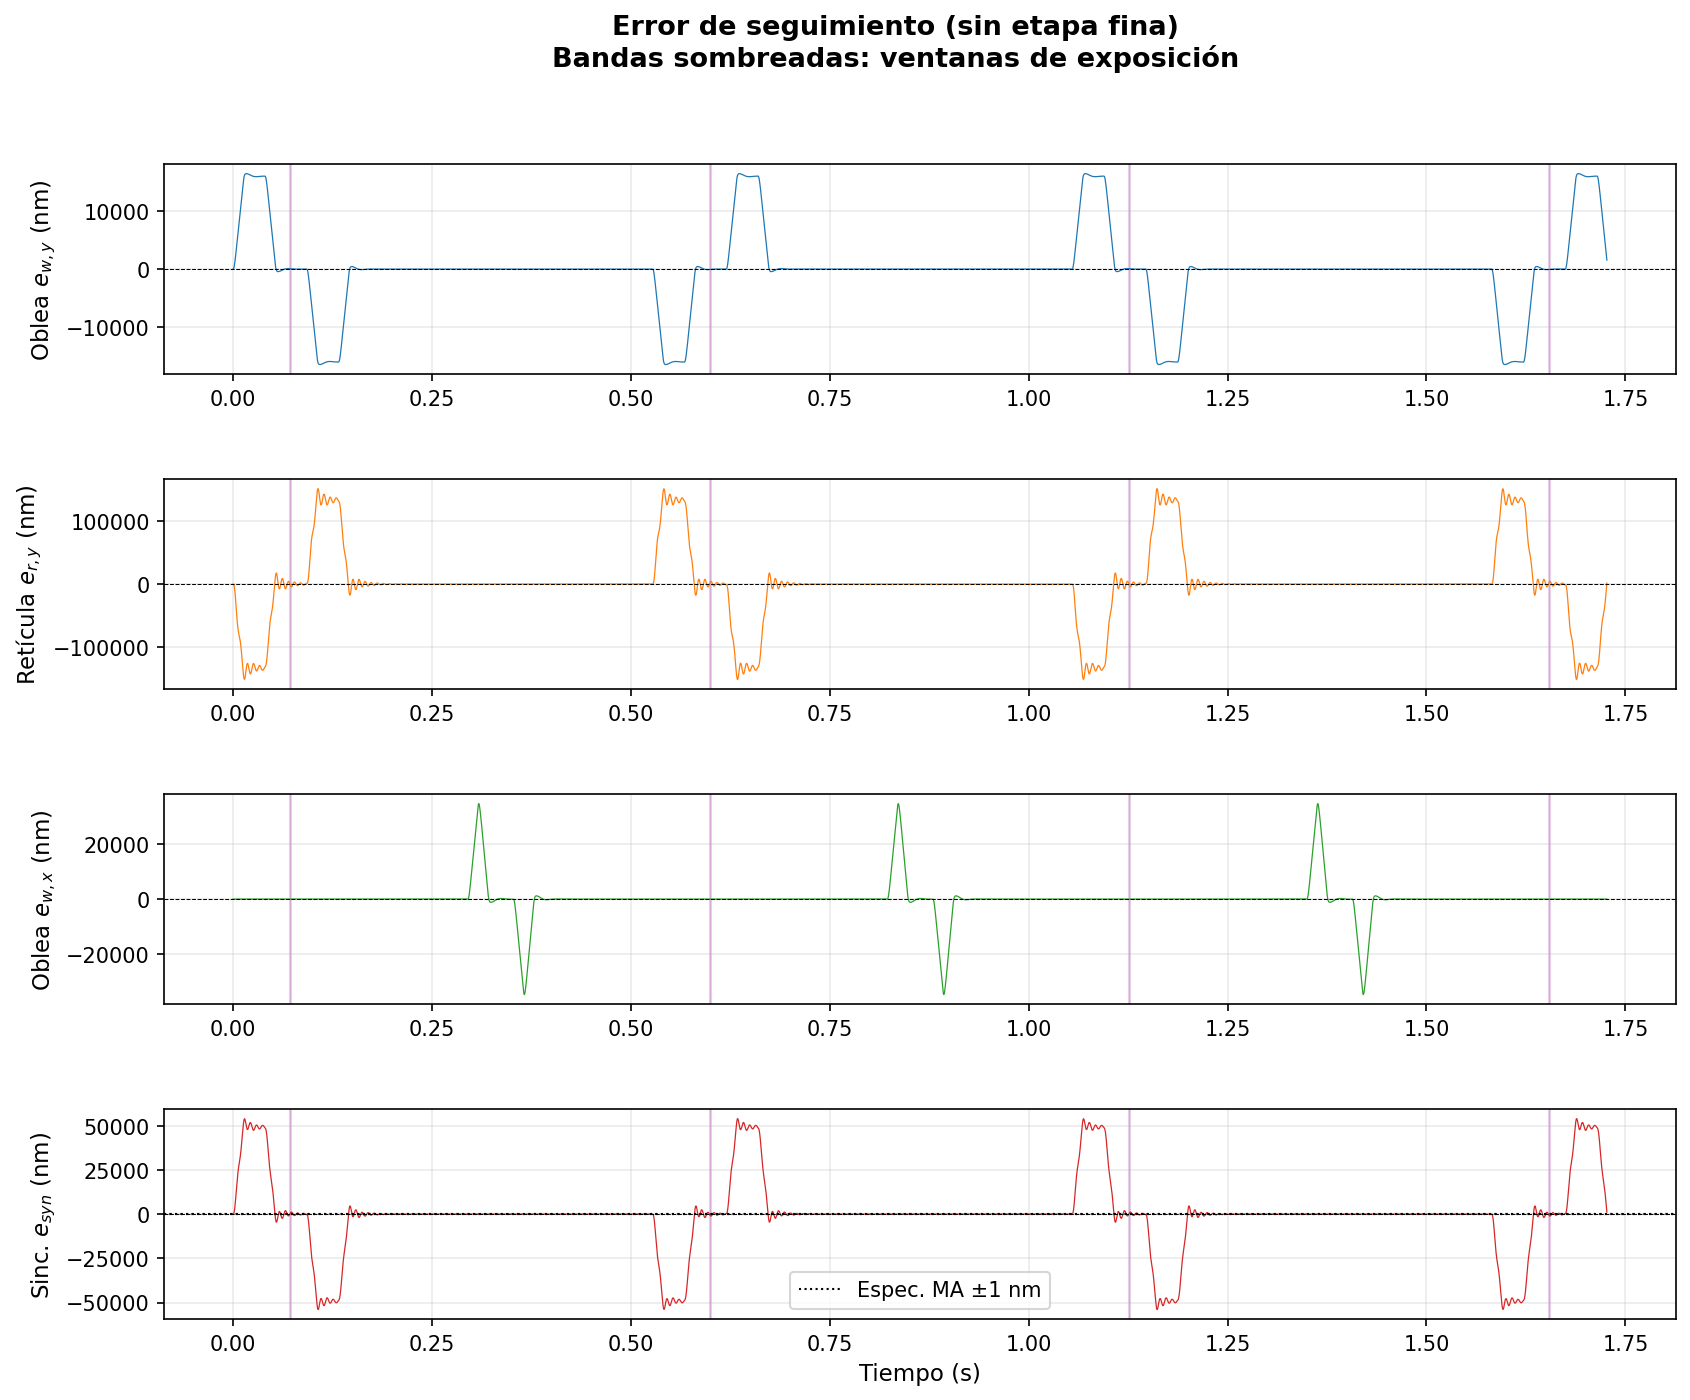
\includegraphics[width=0.46\linewidth,height=0.55\textheight,keepaspectratio]{pictures/sim_tracking.png}\hfill%
        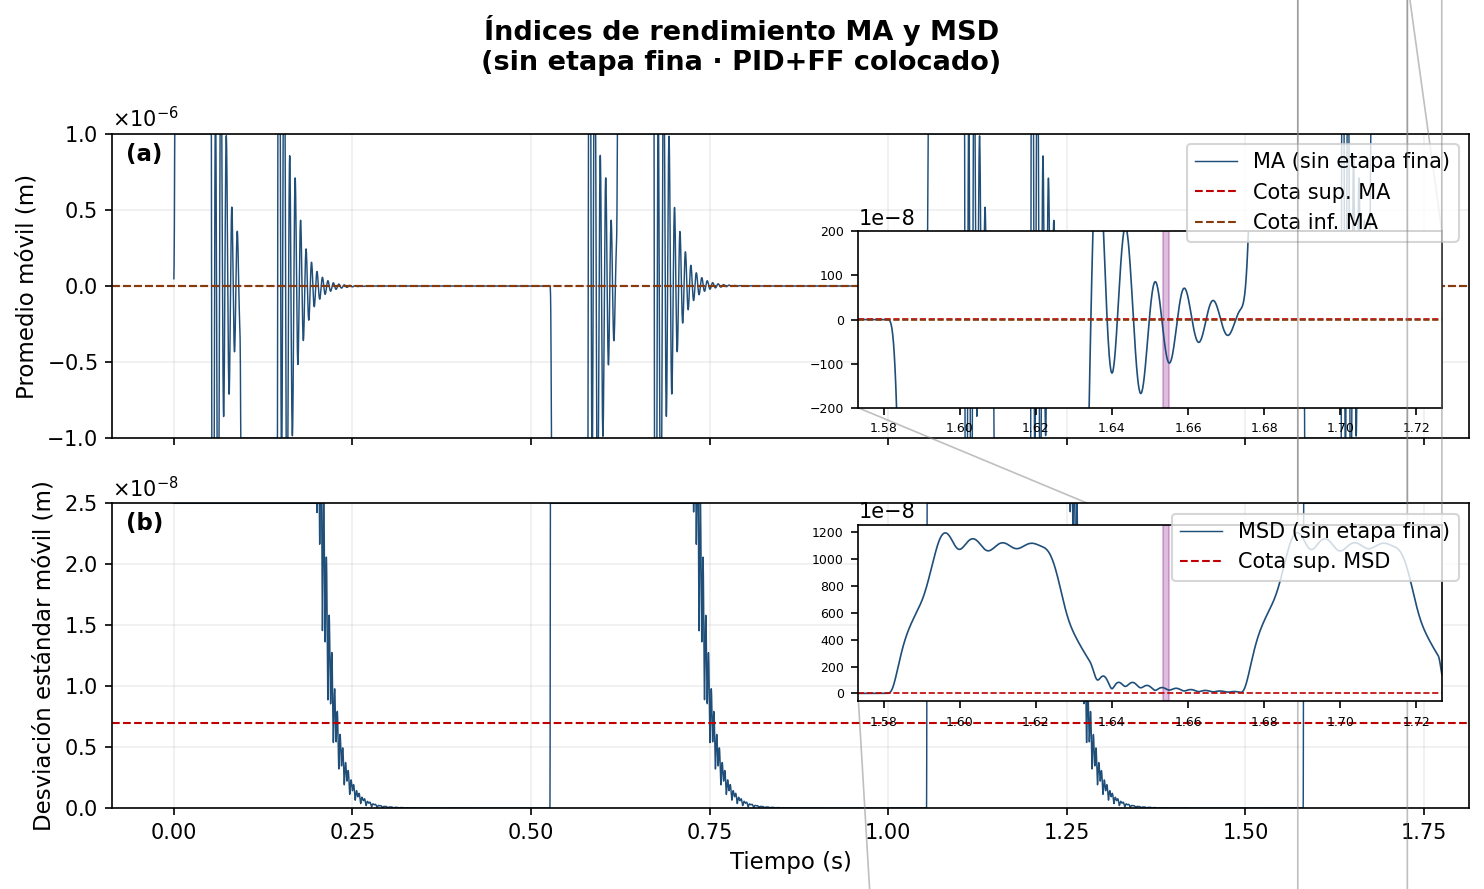
\includegraphics[width=0.46\linewidth,height=0.55\textheight,keepaspectratio]{pictures/sim_ma_msd.png}\\[0.05cm]
        {\footnotesize Error de seguimiento \quad$|$\quad MA y MSD móviles}
    \end{center}
\end{frame}

\begin{frame}{Mapas de defectos y CNN}
    \vspace{0.15cm}
    \begin{columns}[T]
        \column{.26\textwidth}
        \centering
        \small
        \textbf{WM-811K} (\cite{Wu2015_WM811K})\\
        9 clases
        \vspace{0.35cm}
        \begin{tabular}{ll}
            \toprule
            \textbf{Train} & 138\,360 \\
            \textbf{Test} & 34\,590 \\
            \textbf{Arq.} & 3C + 2FC \\
            \textbf{Entrada} & $64{\times}64$ \\
            \textbf{Acc.} & \textbf{96.88\,\%} \\
            \bottomrule
        \end{tabular}

        \column{.36\textwidth}
        \centering
        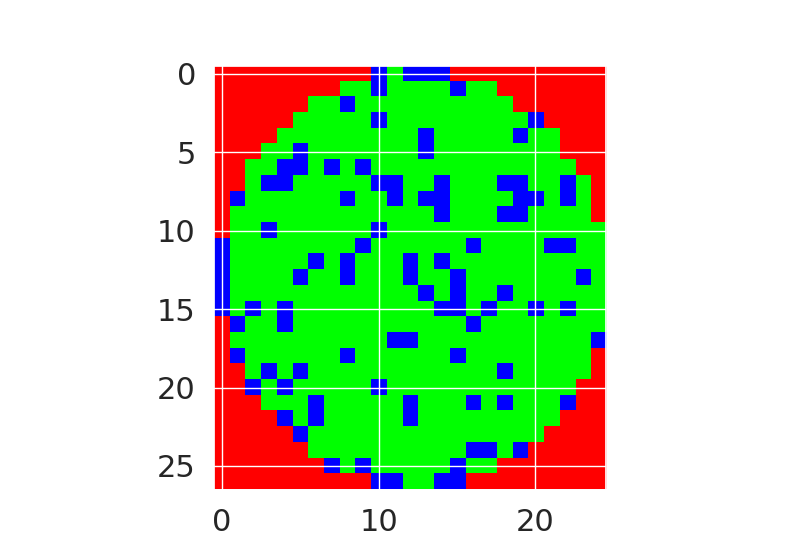
\includegraphics[width=\linewidth,height=0.55\textheight,keepaspectratio]{pictures/wm811k_samples.png}\\[0.05cm]
        {\footnotesize ejemplos por clase}

        \column{.38\textwidth}
        \centering
        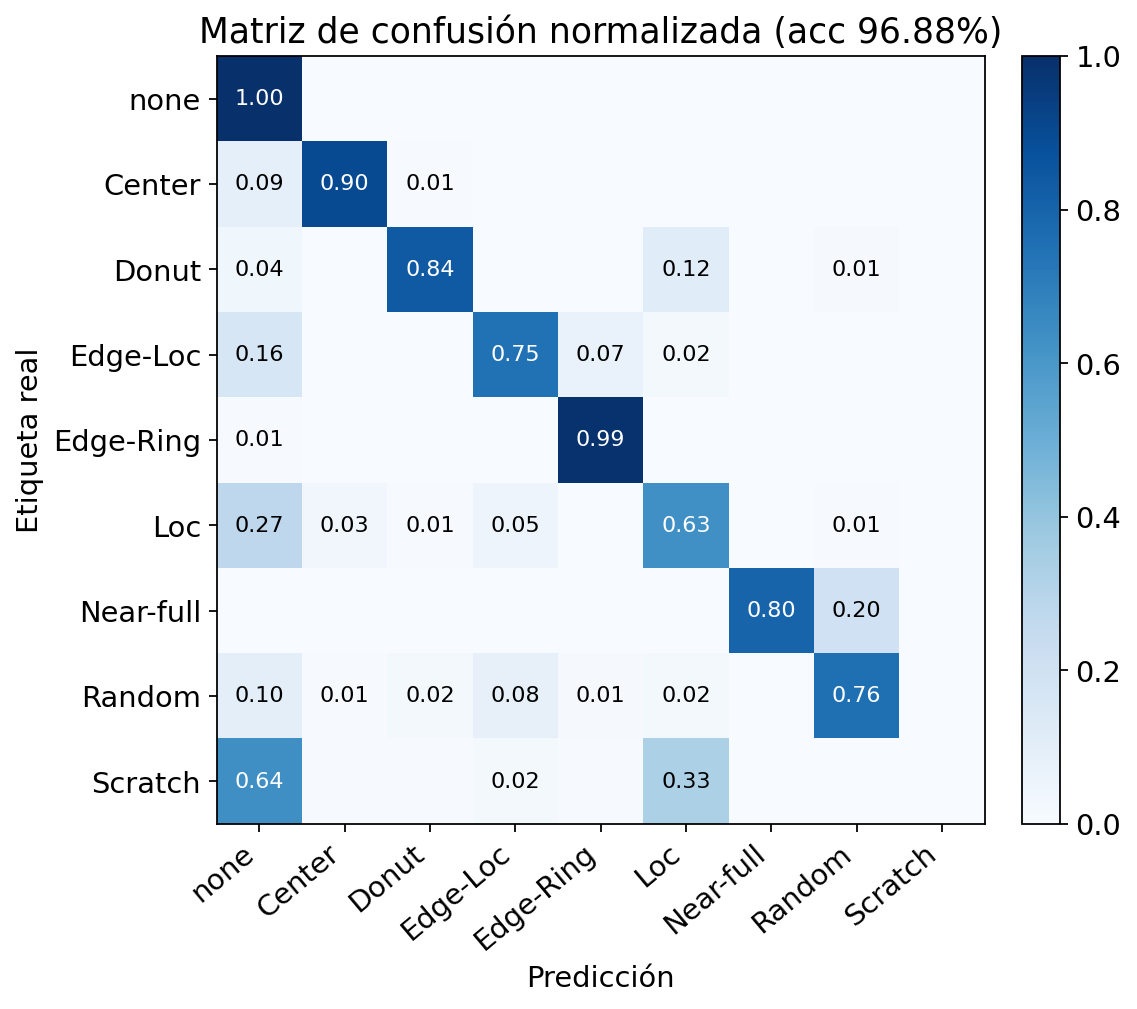
\includegraphics[width=\linewidth,height=0.55\textheight,keepaspectratio]{pictures/cnn_confmat.png}\\[0.05cm]
        {\footnotesize matriz de confusión}
    \end{columns}
\end{frame}

\begin{frame}[fragile]{Conexión trayectoria $\leftrightarrow$ defecto}
    \vspace{0.3cm}
    \begin{center}
    \resizebox{0.92\linewidth}{!}{
    \begin{tikzpicture}[
        block/.style={rectangle, draw=mnnwInk, line width=0.5pt, rounded corners=2pt, minimum height=1.2cm, minimum width=2.5cm, align=center, font=\small},
        oBlock/.style={block, fill=kit-yellow!35},
        modBlock/.style={block, fill=reticleFill},
        yieldBlock/.style={block, fill=waferFill},
        dec/.style={diamond, draw=mnnwInk, line width=0.5pt, aspect=2.2, fill=kit-lightgreen100!25, font=\small, align=center, inner sep=2pt},
        grp/.style={draw=mnnwMute, dashed, line width=0.4pt, rounded corners=4pt, inner sep=12pt},
        flow/.style={-{Stealth[scale=1.1]}, line width=0.7pt, mnnwInk},
        gapflow/.style={-{Stealth[scale=1.1]}, line width=1.1pt, kit-red100, dashed}
    ]
        \node[modBlock] (traj) {Trayectoria\\(cuarto orden)};
        \node[modBlock, right=0.7cm of traj] (mass) {Simulación\\multicuerpo};
        \node[modBlock, right=0.7cm of mass] (err) {Error\\MA / MSD};

        \node[yieldBlock, right=1.2cm of err] (map) {Mapa de\\defectos};
        \node[yieldBlock, right=0.7cm of map] (cls) {CNN\\$\widehat{P}_{\text{defecto}}$};

        \node[oBlock, below=1.6cm of mass] (pso) {Algoritmo bio-inspirado\\sobre $(v,a,j,s)_{\max}$};
        \node[dec, right=1.2cm of pso] (cost) {Función\\de costo};

        \draw[flow] (traj) -- (mass);
        \draw[flow] (mass) -- (err);
        \draw[gapflow] (err) -- (map) node[midway, above, text=kit-red100, font=\small\bfseries, fill=white, inner sep=1pt] {brecha};
        \draw[flow] (map) -- (cls);
        \draw[flow] (cls.south) |- (cost.east);
        \draw[flow] (cost) -- (pso);
        \draw[flow] (pso.west) -| (traj.south);

        \node[grp, fit={(traj) (mass) (err)}, label={[font=\small\bfseries]above:Objetivo 1 --- seguimiento}] {};
        \node[grp, fit={(map) (cls)}, label={[font=\small\bfseries]above:Objetivo 2 --- vínculo predictivo}] {};
        \node[grp, fit={(pso) (cost)}, label={[font=\small\bfseries]below:Objetivo 3 --- perfiles óptimos}] {};
    \end{tikzpicture}
    }
    \\[0.3cm]
    {\small \textcolor{kit-red100}{\textbf{Brecha:}} cerrar el mapeo error $\to$ mapa vía \textit{dose mapping} (física) o \textit{paired learning} (datos).}
    \end{center}
\end{frame}

\begin{frame}[fragile]{Trayectorias de alto orden}
    \vspace{0.2cm}
    \begin{columns}
        \column{.55\textwidth}
        \centering\small
        \textit{Snap} acotado $\Rightarrow$ menor error de \textit{overlay} (\cite{Al-Rawashdeh2023_Trajectories}).
        \vspace{0.5cm}

        {\small
        \begin{tabular}{ll}
            \toprule
            \textbf{Método} & \textbf{Fuente} \\
            \midrule
            Polinomios segmentados & \cite{Lambrechts2003_Trajectories} \\
            \textit{Input shaping} & convolucional \\
            Cuadrado / bisel / meandro & \cite{Al-Rawashdeh2023_Trajectories} \\
            \bottomrule
        \end{tabular}}
        \column{.45\textwidth}
        \begin{center}
          \begin{tikzpicture}[scale=0.85,
            every node/.style={font=\footnotesize},
            wafer/.style={draw=kit-blue100, line width=0.6pt, fill=kit-blue!5},
            die/.style={draw=mnnwInk, line width=0.3pt, fill=white, postaction={pattern=north east lines, pattern color=mnnwMute!40}},
            square/.style={draw=mnnwInk, line width=0.8pt},
            fillet/.style={draw=mnnwSignal, line width=0.8pt},
            meander/.style={draw=opticsEdge, line width=0.8pt},
            axis/.style={draw=mnnwInk, -Stealth}
          ]

            % Wafer boundary
            \draw[wafer] (0,0) circle (2.2cm);

            % Grid of dies clipped to wafer
            \begin{scope}
              \clip (0,0) circle (2.2cm);
              \foreach \x in {-1.75,-1.25,...,1.75} {
                \foreach \y in {-1.75,-1.25,...,1.75} {
                  \draw[die] (\x-0.2,\y-0.2) rectangle (\x+0.2,\y+0.2);
                }
              }
            \end{scope}

            \draw[mnnwInk, line width=0.8pt, dashed] (-1.25, -1.75) -- (-1.25, -1.25);

            % Square Profile
            \draw[square] (-1.25, -1.25) -- (-1.25, -1.0) -- (-0.75, -1.0) -- (-0.75, -1.25);

            % Fillet Profile
            \draw[fillet] (-1.25, -1.25) -- (-1.25, -1.12)
                          arc(180:90:0.12) -- (-0.87, -1.0)
                          arc(90:0:0.12) -- (-0.75, -1.12)
                          -- (-0.75, -1.25);

            % Meander Profile
            \draw[meander] (-1.25, -1.25) to[out=90, in=180] (-1.0, -1.0) to[out=0, in=90] (-0.75, -1.25);

            \draw[mnnwInk, line width=0.8pt, dashed] (-0.75, -1.25) -- (-0.75, -1.75);

            \begin{scope}[shift={(-2.4, -2.7)}]
              \draw[square]  (0, 0.55) -- (0.35, 0.55) node[right, font=\footnotesize] {Cuadrado};
              \draw[fillet]  (0, 0.27) -- (0.35, 0.27) node[right, font=\footnotesize] {Bisel};
              \draw[meander] (0, 0.00) -- (0.35, 0.00) node[right, font=\footnotesize] {Meandro};
            \end{scope}

            \draw[axis] (0,0) -- (0.4,0) node[right] {$x$};
            \draw[axis] (0,0) -- (0,0.4) node[above] {$y$};

          \end{tikzpicture}
        \end{center}
    \end{columns}
\end{frame}

\section{Trabajo posterior}

\begin{frame}[fragile]{Siguientes pasos}
    \vspace{0.5cm}
    \begin{center}
    \begin{tikzpicture}[
        every node/.style={font=\small},
        stp/.style={draw=opticsEdge, line width=0.7pt, rounded corners=2pt, fill=opticsFlex, minimum width=2.9cm, minimum height=2.0cm, align=center},
        hi/.style ={draw=kit-red100, line width=1.0pt, rounded corners=2pt, fill=kit-red!8, minimum width=2.9cm, minimum height=2.0cm, align=center},
        ar/.style={-Stealth, line width=0.9pt, opticsEdge}
    ]
        \node[stp] (a) {\textbf{1.}\\Controlador\\no lineal\\\footnotesize\cite{Heertjes2025_NonlinearControl}};
        \node[stp, right=0.55cm of a] (b) {\textbf{2.}\\Estimador de\\parámetros};
        \node[hi,  right=0.55cm of b] (c) {\textbf{3.}\\\textbf{Mapeo}\\error $\leftrightarrow$ defecto\\\footnotesize\cite{Yang2018_Yield}};
        \node[stp, right=0.55cm of c] (d) {\textbf{4.}\\Comparar\\órdenes de\\trayectoria\\\footnotesize\cite{Al-Rawashdeh2023_Trajectories}};
        \draw[ar] (a) -- (b);
        \draw[ar] (b) -- (c);
        \draw[ar] (c) -- (d);
    \end{tikzpicture}
    \end{center}
    \vspace{0.7cm}
    \begin{center}
    {\large\itshape Gracias por su atención.}
    \end{center}
\end{frame}

\appendix
\beginbackup

\begin{frame}[fragile]{Apéndice: esquema multi-cuerpo detallado}
    \begin{center}
        \begin{turn}{90}
        \detailedMultibodyFigure
        \end{turn}
    \end{center}
\end{frame}

\begin{frame}[allowframebreaks]{Referencias}
\printbibliography
\end{frame}
\backupend

\end{document}
